\documentclass[12pt, letter, landscape]{article}

% \usepackage[paperheight=17in,paperwidth=11in,margin=0.5in]{geometry}

% Required for inserting images
\usepackage{graphicx}
% Required for tracking version history
\usepackage{vhistory}
% Required for adding affliation to author(s)
\usepackage{authblk}
% Required for hyperref and url
\usepackage[colorlinks=true,linkcolor=blue,urlcolor=blue]{hyperref}
\usepackage{titlesec}

% adapted from https://www.reddit.com/r/LaTeX/comments/81ugpm/remove_chapter_from_from_chapter_headings/
\titleformat{\chapter}{\huge\normalfont\bfseries}{\thechapter}{1em}{}

% adapted from https://tex.stackexchange.com/questions/593640/disable-hyperref-link-for-single-footnote/
\newcommand\blfootnote[1]{
  \begin{NoHyper}
  \renewcommand\thefootnote{}\footnote{#1}
  \addtocounter{footnote}{-1}
  \end{NoHyper}
}

\begin{document}

\title{Stable Diffusion XL Turbo UNet FP32 512x512}
\author{Shamith Achanta}
\date{06.03.2024}

\maketitle

\section{Assumptions}
\begin{itemize}
	\item The set of operators that have the same output memory size are likely to be fused and computed as a single operator to reduce the number of times the output needs to be read from memory. Hence, the total memory of the blocks in red are not counted in the analysis.
	\item The on-chip memory on the NPU is a parameter. In this analysis, the on-chip memory is set to 4 MB and data (weights + output) with memory size greater than the on-chip memory will need to be stored in the Last-level cache (if-any) or Main Memory
\end{itemize}

\begin{figure}[h]
\caption{Optimization 1}
\centering
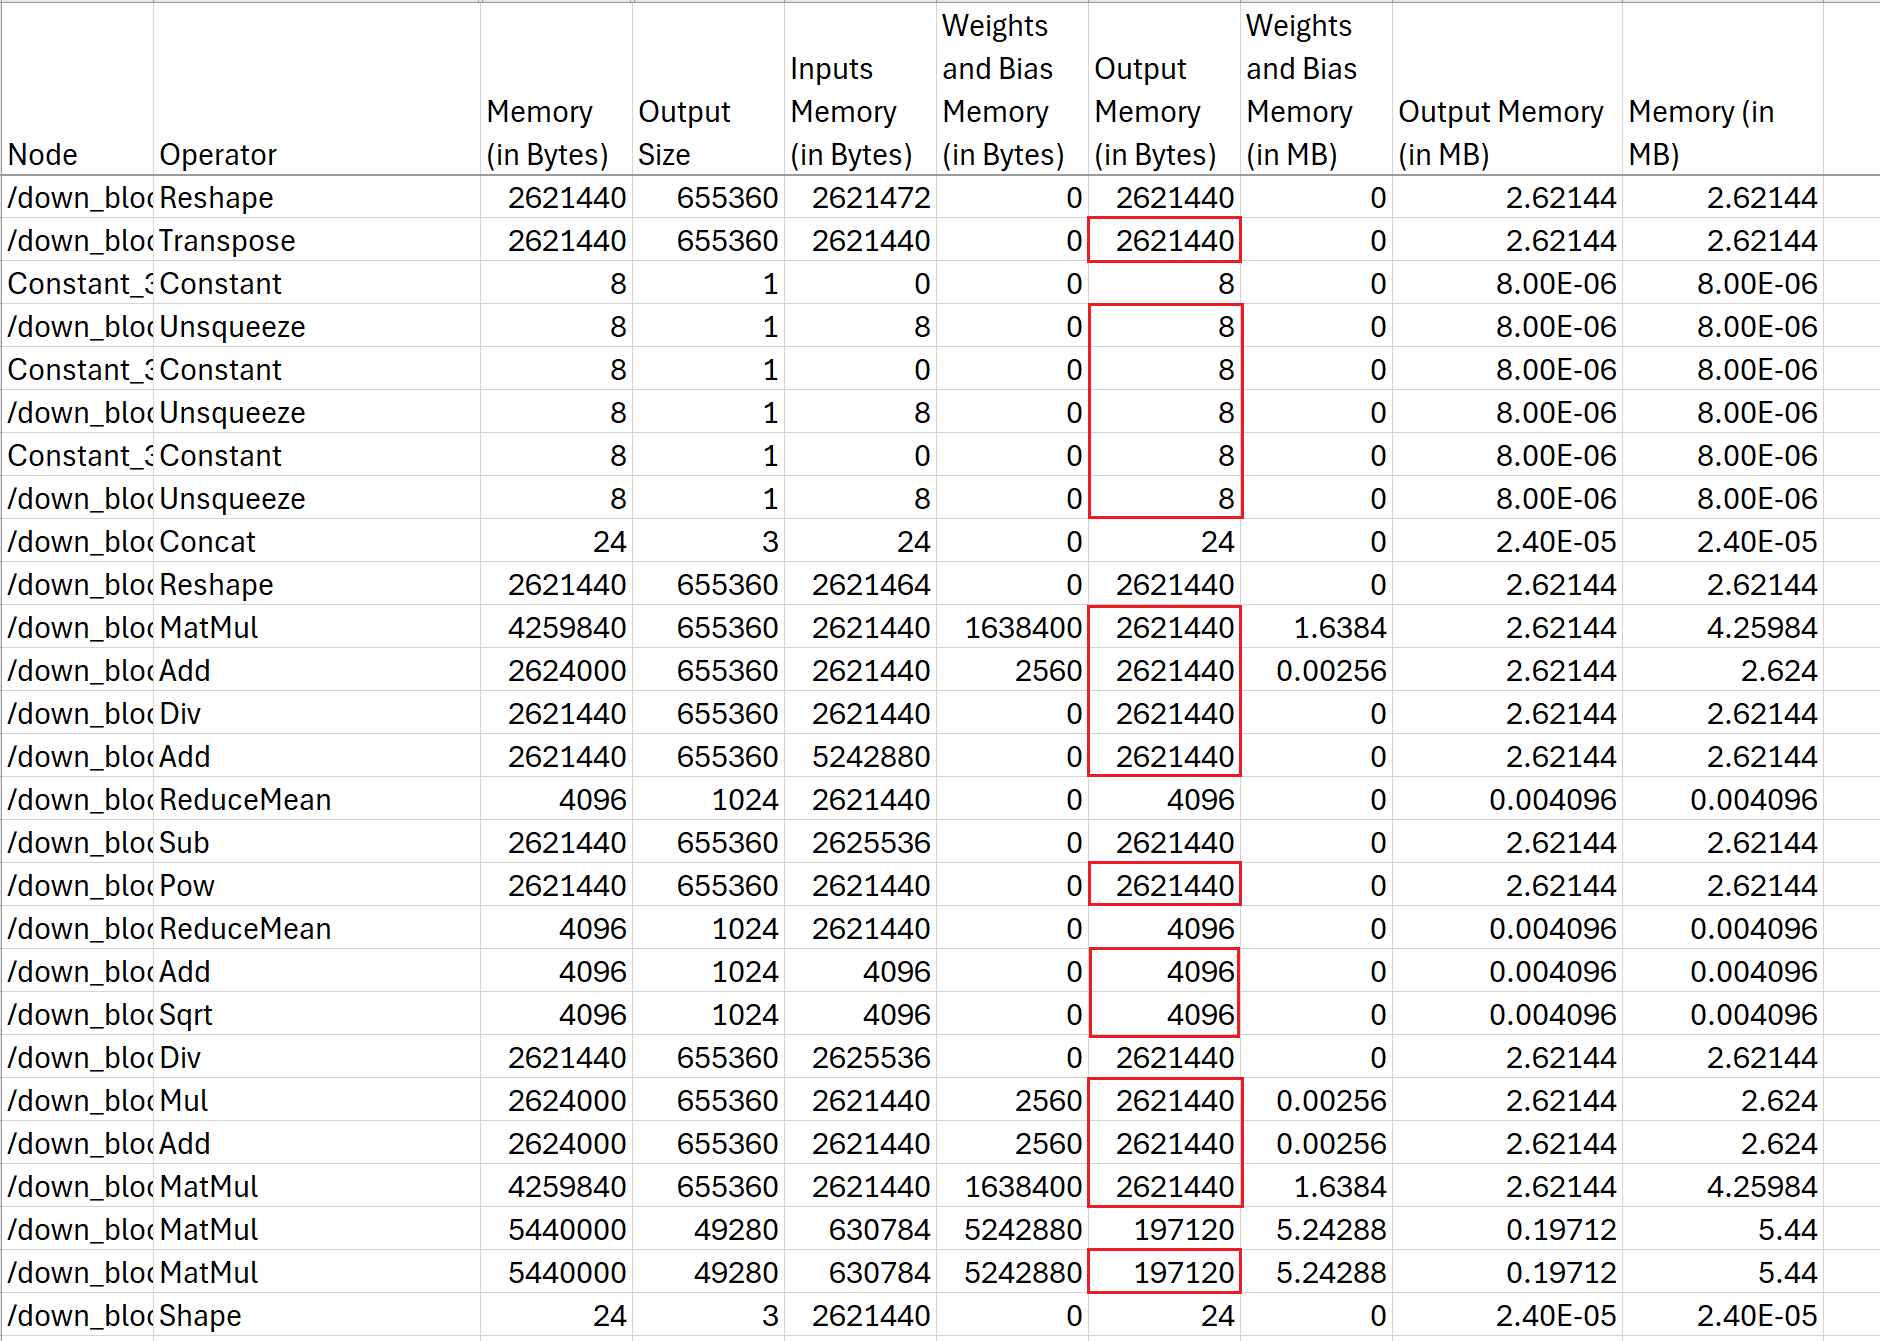
\includegraphics[width=1.1\textwidth]{sdxl_turbo_unet_analysis_optimization1}
\end{figure}

\clearpage

\section{Operator Memory Distribution}
\begin{itemize}
	\item Output + Weight matrices above on-chip memory size for an operator need to be stored in the Main Memory or last-level cache (if-any)
	\item Total memory of all operators that have memory size $>$ on-chip memory size is 10 GB
\end{itemize}

\begin{figure}[h]
\caption{Operator Memory Distribution}
\centering
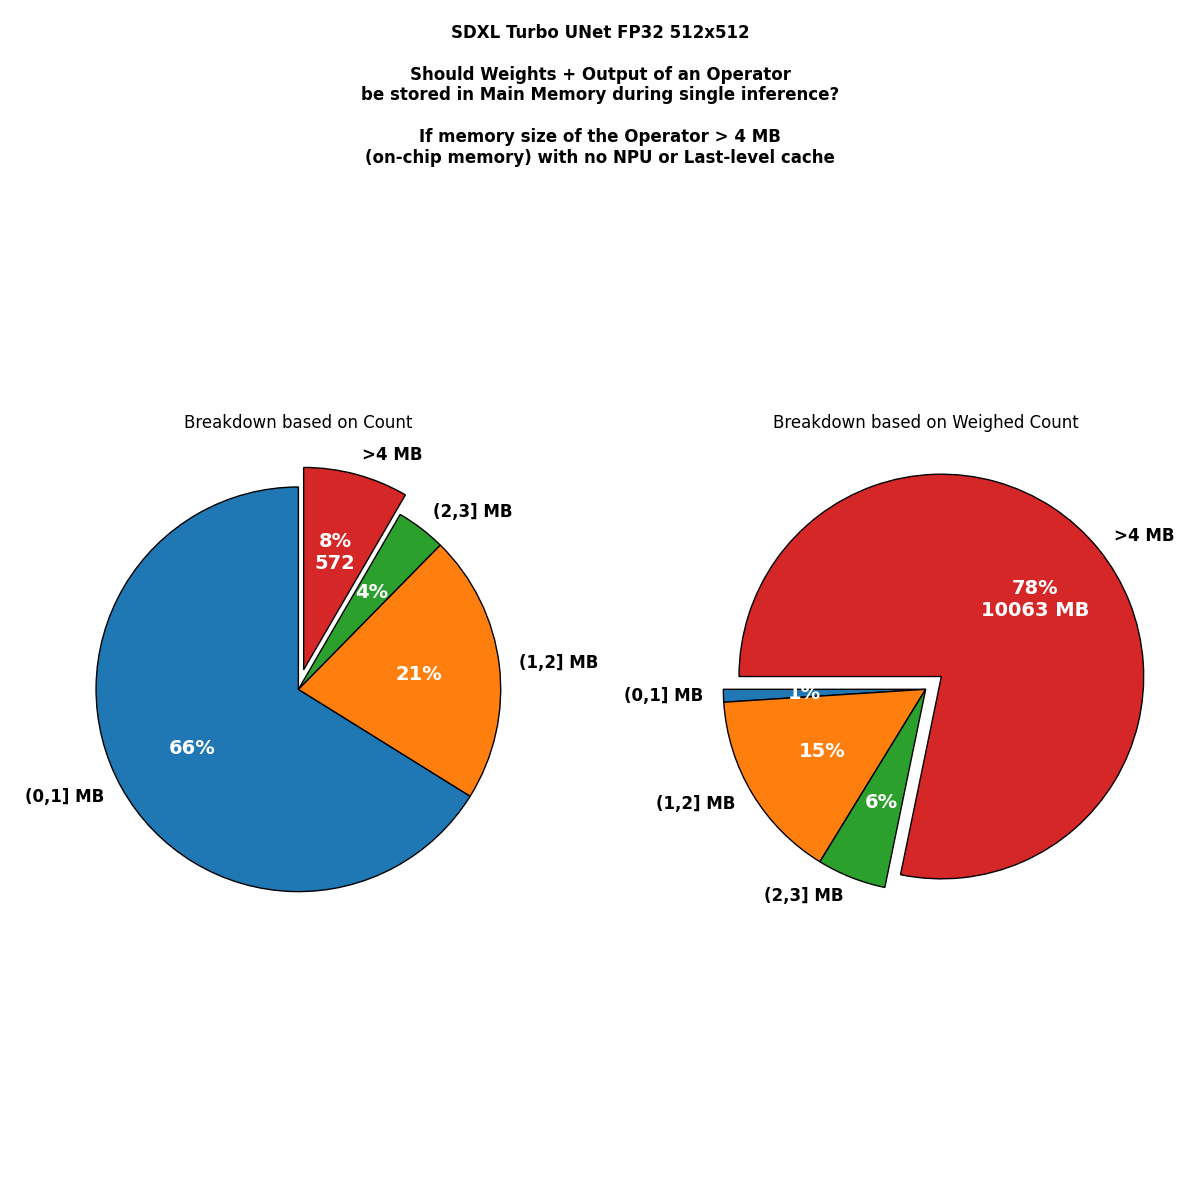
\includegraphics[width=1.1\textwidth]{sdxl_turbo_unet_fp32_512x512_4mb_pie_plot}
\end{figure}

\clearpage

\section{Memory Requirement of Individual Operators}
Operators that have weights + output memory size $>$ on-chip memory size
\begin{figure}[h]
\caption{Memory Requirement of Individual Operators $>$ 4 MB}
\centering
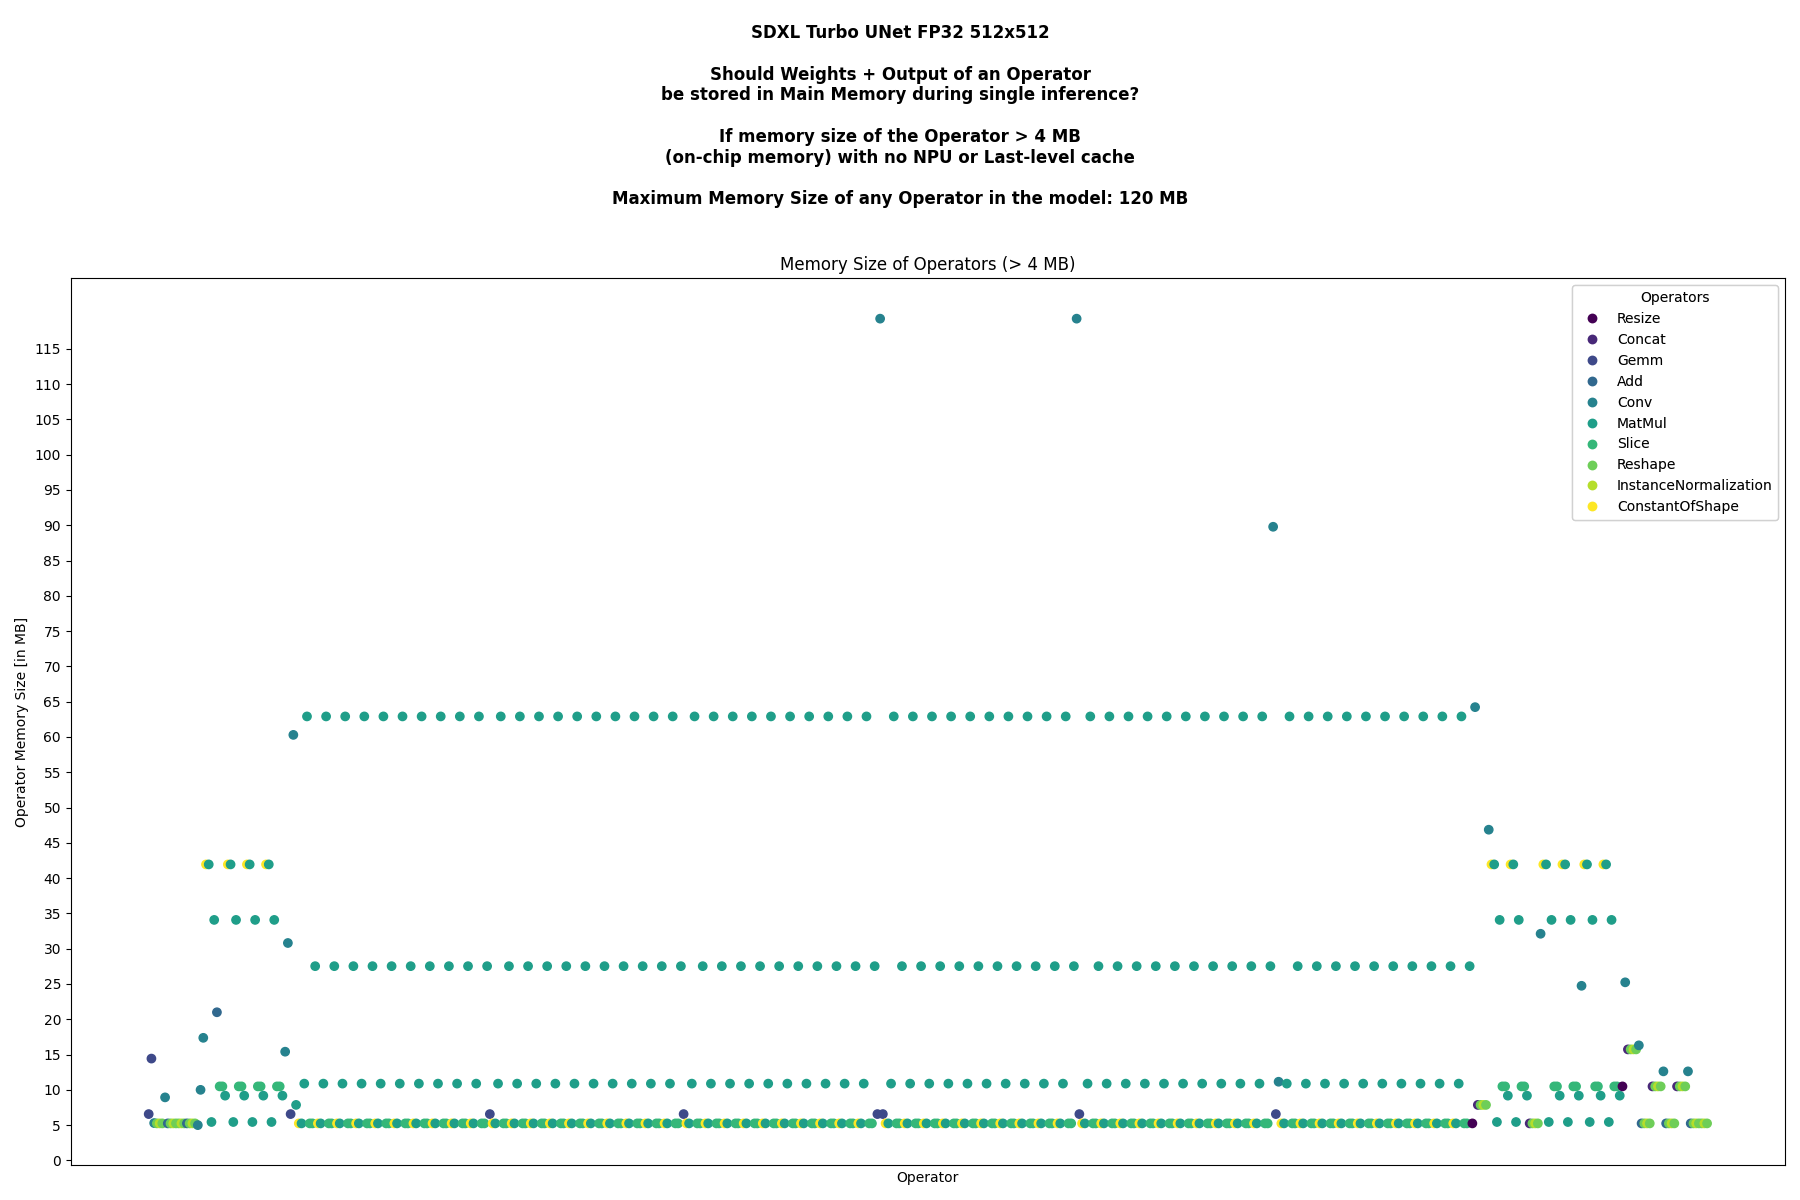
\includegraphics[width=1.1\textwidth]{sdxl_turbo_unet_fp32_512x512_4mb_operators_plot}
\end{figure}

\clearpage

\begin{figure}[h]
\caption{Memory Requirement of Individual Operators $>$ 9 MB}
\centering
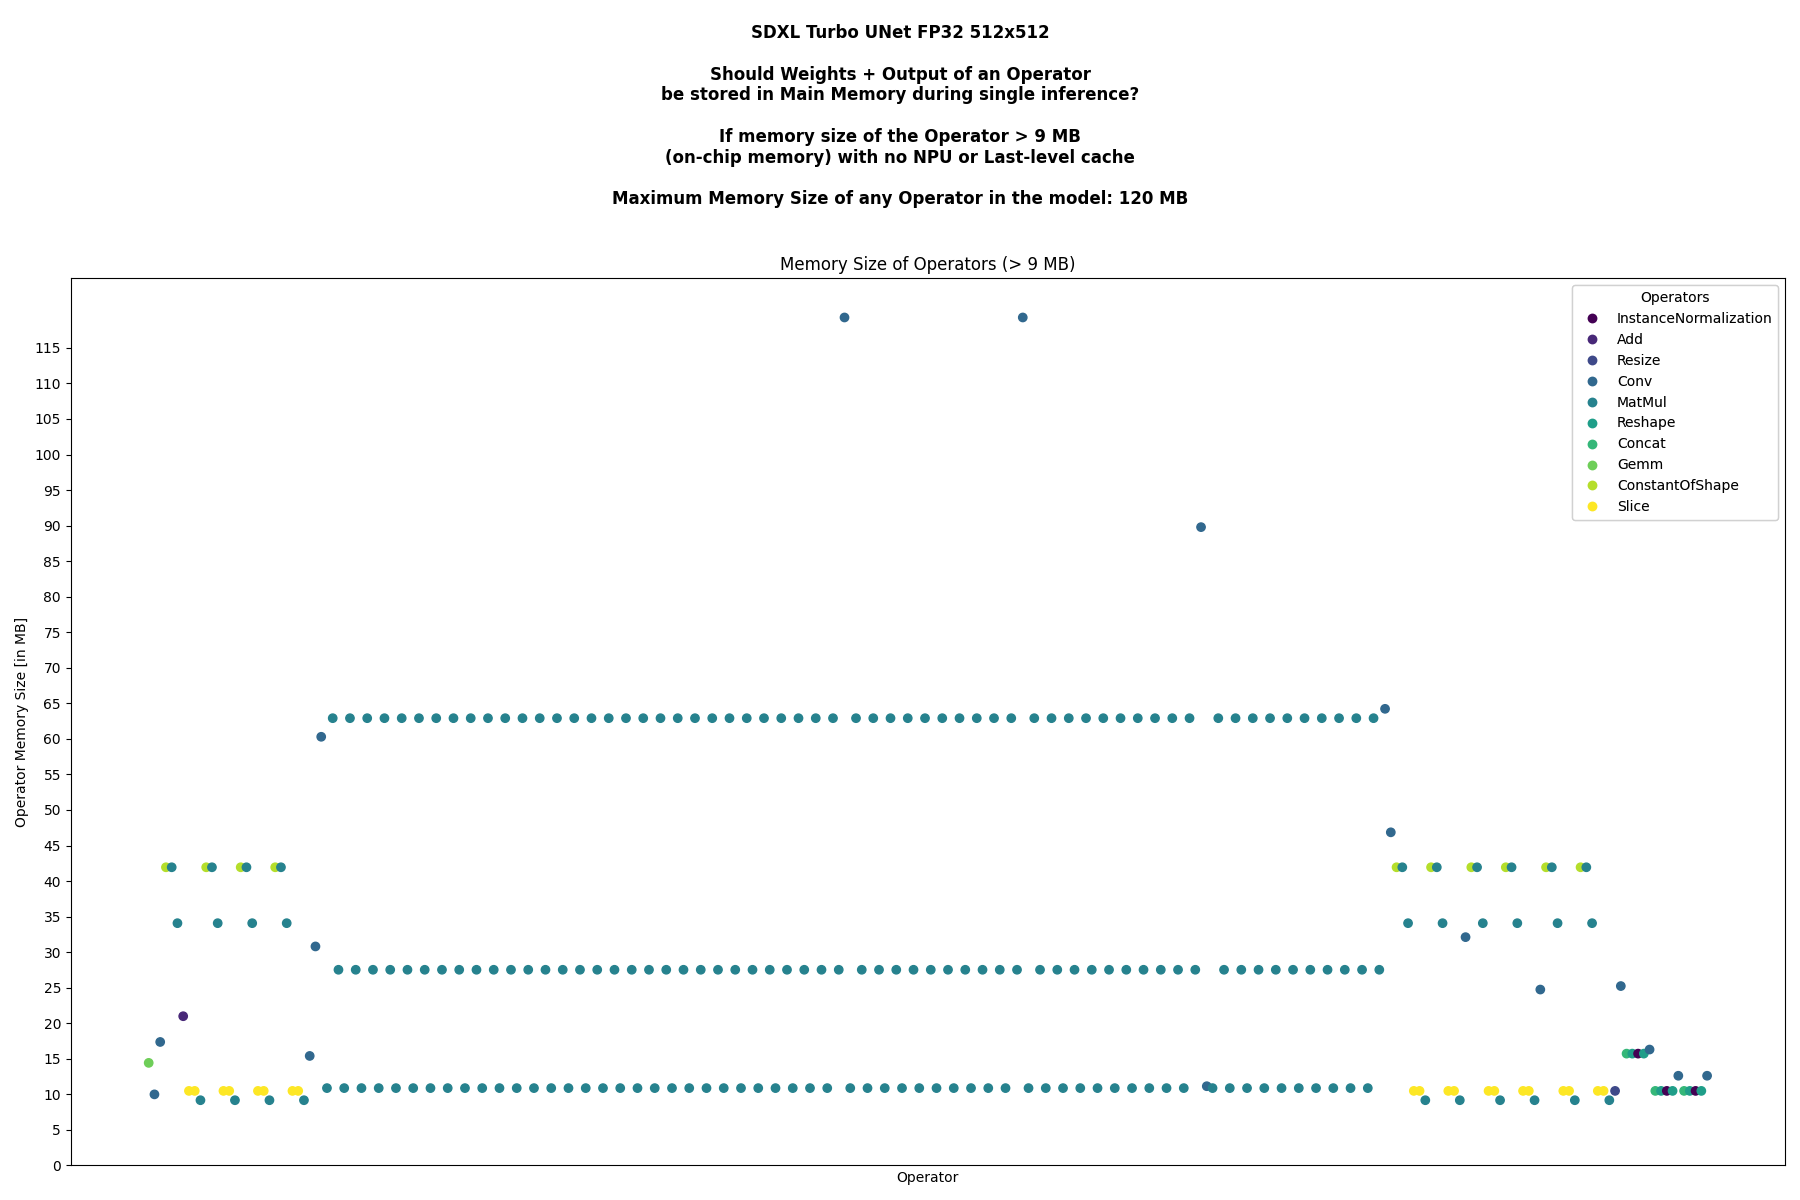
\includegraphics[width=1.1\textwidth]{sdxl_turbo_unet_fp32_512x512_9mb_operators_plot}
\end{figure}

\clearpage

\end{document}
